\documentclass[11pt]{book}
\usepackage[T1]{fontenc}
\usepackage{textcomp}
\usepackage{listings}
\usepackage{url}


\lstset{upquote=true}

\newcommand{\legionbook}[1]{{\tt LegionManual/Examples/#1}}
\newcommand{\Cpp}{C++}

\begin{document}

\title{Programming with Legion}
\author{Alex Aiken \and Michael Bauer}
\date{June 21, 2019}
\maketitle

\subsection*{Preface}
\addcontentsline{toc}{subsection}{Preface}

The first paper describing the Legion programming model
was published in 2012 \cite{Legion12}.  Since then, there has been
enormous progress and many people have contributed to
the project.  Throughout this period new application developers have
learned Legion through a combination of examples, lore from other
members of the project, research papers and reading the source code of
the Legion implementation.  The intention here is to put down in 
a systematic fashion what a programmer who wants to use
Legion to develop high performance applications needs to know.

This book is intended to be a combination tutorial, rationale and
manual.  The first part is the tutorial and rationale, laying out in some
detail what Legion is and why it is that way.  The second part is the manual, which describes
each of the API calls for the Legion \Cpp\ runtime.

The example programs and configuration files referred to in this book can be found in the directory
\legionbook{} included in the Legion distribution.

This book is incomplete and will remain incomplete for
some time to come.  But on the theory that partial documentation is better than no
documentation, the manual is being made available while it is
still in progress in the hope that it will be useful to new Legion
programmers.  Please report any errors or other issues to {\tt
  aiken@cs.stanford.edu}. \\[2in] Alex Aiken\\ Stanford, CA \\ June
2019

\tableofcontents

\part{Legion Runtime Tutorial}


\chapter{Installation}
\label{chap:start}

The Legion homepage is \url{legion.stanford.edu}.  Here you will find
links to everything associated with the project, including a set of
tutorials that are distinct from this manual.  The Legion distribution is at
\url{https://github.com/StanfordLegion/legion}.  The distribution has been
tested on Linux machines and Mac OS X.  To install, in a shell type
\begin{lstlisting}[language=bash]
> cd DIR
> git clone https://github.com/StanfordLegion/legion
\end{lstlisting}
where {\tt DIR} is a directory of your choice.  This command creates 
the directory {\tt DIR/legion}.  To complete the installation,
set the environment variable {\tt LG\_RT\_DIR} to {\tt DIR/legion/runtime}.
For {\tt bash} users, an example {\tt .bashrc} is included in
\legionbook{Installation}.

\section{Regent}

If only the Legion \Cpp\ runtime is desired, there is no need to install Regent, the companion
Legion programming language, and this section can be ignored.  To install Regent, download LLVM
from the following URL
{\small\url{http://llvm.org/releases/3.4.2/clang+llvm-3.4.2-x86_64-apple-darwin10.9.xz}}
and extract it in a directory of your choice:
{\small
\begin{verbatim}
> cd DIR
> tar xf http://llvm.org/releases/3.4.2/clang+llvm-3.4.2-x86_64-apple-darwin10.9.xz
\end{verbatim}
}
You must then put the LLVM {\tt bin} directory in your search {\tt
  PATH} and the LLVM {\tt lib} in yor {\tt DYD\_LIBRARY\_PATH}.  The
example {\tt .bashrc} file in \legionbook{Installation} contains the
necessary commands for {\tt bash} users.



\chapter{Tasks}
\label{chap:tasks}

% Set up the listing configuration for everything
\lstset{
  captionpos=b,
  language=C++,
  basicstyle=\scriptsize,
  numbers=left,
  numberstyle=\tiny,
  columns=fullflexible,
  stepnumber=1,
  escapechar=\#,
  keepspaces=true,
  literate={<}{{$\langle$}}1 {>}{{$\rangle$}}1,
  %xleftmargin=15pt,
}

The Legion runtime is a \Cpp\ library, and
Legion programs are just C++ programs that use the Legion runtime API.
One important consequence of this design is that almost all Legion decisions
(such as what data layout to use, in which memories to place data and on which
processors to run computations) are made dynamically,  during the execution of 
a Legion application.  Dynamic decision making provides maximum flexibility, 
allowing the runtime's decisions to be reactive to the current state of the computation.
Implementing Legion as a \Cpp\ library also allows high performance \Cpp\ code
(e.g., vectorized kernels) to be used seamlessly in Legion applications.

In Legion, {\em tasks} are distinguished functions with a specific signature.
Legion tasks have several important properties:
\begin{itemize}
\item Tasks are the unit of parallelism in Legion; all parallelism occurs because tasks are executed in parallel.

\item Tasks have {\em variants} specific to a particular kind of {\em processor} (most commonly CPUs or GPUs, but there is also experimental support for FPGAs) and 
memory layout of the task's arguments.  A task may have multiple variants.

\item Once a task begins execution on a processor, that task will execute in its entirety on that processor---tasks do
not migrate mid-computation.  

\end{itemize}


\begin{figure}
  {\small
    \lstinputlisting{Examples/Tasks/sum/sum.cc}
  }
\caption{\legionbook{Tasks/sum/sum.cc}}
\label{fig:simple}
\end{figure}

Figure~\ref{fig:simple} shows a very simple, but complete, Legion program for summing
the first 1000 positive integers (also available as {\tt sum.cc} in \legionbook{Tasks}).
This example, like every other example in this manual, can be run by first setting an environment variable to point to the Legion runtime
\begin{verbatim}
export LG_RT_DIR="...path to legion directory.../legion/runtime"
\end{verbatim}
and then typing {\tt make} in the directory containing the example.

At a high level, every Legion program has three components:
\begin{itemize}
\item The id of the top-level task must be set with Legion's {\em high level runtime}.  The top-level
task is the initial task that is called when the Legion runtime starts.
\item Every task and its task id must be registered with the high level runtime.  Currently all tasks
must be registered before the runtime starts.
\item The start method of the high level runtime is invoked, which in turn calls the top-level task.
Note that by default this call does not return---the program is terminated when the start method terminates.
\end{itemize}
In Figure~\ref{fig:simple}, these three steps are the three statements of {\tt main}.  
The only task in this program is {\tt sum\_task}, which is also the top-level task invoked when the
Legion runtime starts up.  Note that the program does not say where the task is executed; that decision is made
at runtime by the {\em mapper} (see Chapter~\ref{chap:mapping}).  Note also that tasks can perform almost arbitrary
\Cpp\ computations.  In the case of {\tt sum\_task}, the computation performed is very simple, but in general tasks
can call ordinary \Cpp\ functions, including allocating and deallocating memory.  Tasks must not, however,
call directly into other packages that provide parallelism or concurrency.  Interoperation with OpenMP and MPI is
possible but must be done in a standardized way (see Chapter~\ref{chap:interop}).  

As mentioned above, every task must be registered with the Legion runtime before
the runtime's {\tt start} method is called.  Registration passes several arguments about a
task to the runtime:
\begin{itemize}
\item The name of the task is a template argument to the {\tt register\_legion\_task} method.

\item The task ID is the first (regular) argument.

\item The kind of processor the task can run on is the second argument.  The most important options are
{\em latency optimized cores} or CPUs (constant {\tt LOC}) and {\em throughput optimized cores} or GPUs
(constant {\tt TOC}).

\item Two boolean flags, the first of which indicates whether the task can be used in a single task
launch and the second of which indicates whether the task can be used in a multiple (or {\em index}) task
launch.
\end{itemize}

We will see shortly that tasks can call other tasks and pass
those tasks arguments and return results.  Because the called task may
be executed in a different address space than the caller, arguments
passed between tasks must not contain \Cpp\ pointers, as these will
not make sense outside of the address space in which they were
created.  Neither should tasks refer to global variables. A common
programming error for beginning Legion programmers is to pass
\Cpp\ pointers or references between tasks, or to refer to global
variables from within tasks.  As long as all the tasks are mapped to a
single node (i.e., the same address space) the program is likely to
work, but when efforts are made to scale up the application by running
on multiple nodes, \Cpp\ crashes result from the wild pointers or
references to distinct instances of global variables of the same name
in different address spaces.  Legion provides its own abstractions for
passing data structures between tasks (see
Chapter~\ref{chap:regions}).

All tasks have the same input signature as {\tt sum\_task}:
\begin{itemize}

\item {\tt const Task *task}: An object representing the task itself. 

\item {\tt const std::vector<PhysicalRegion> \&regions}: A vector of {\em physical region instances}.  This argument is the
primary way to pass data between tasks (see Chapter~\ref{chap:regions}).

\item {\tt Context ctx}: Every task is called in a context, which contains metadata for the task.  Application programs
should not directly manipulate the context.

\item {\tt Runtime *runtime}: A pointer to the runtime, which gives the task access to the Legion runtime's methods.

\end{itemize}

\section{Subtasks}
\label{sec:subtasks}


\begin{figure}
  {\small
    \lstinputlisting{Examples/Tasks/subtasks/subtasks.cc}
    }
\caption{\legionbook{Tasks/subtasks/subtasks.cc}}
\label{fig:subtask}
\end{figure}



Task can call other tasks, known as {\em subtasks}.  We also refer to
the calling task as the {\em parent task} and the called task as the
{\em child task}.  Two or more child tasks of the same parent task are
{\em sibling tasks}.  Figure~\ref{fig:subtask} shows the definition of
the parent task and the child task from the example
\legionbook{Tasks/subtask/subtask.cc}.

Consider the parent task {\tt top\_level\_task}.  There are two steps
to executing a subtask.  First, a {\tt TaskLauncher} object is
created.  The {\tt TaskLauncher}
constructor takes two arguments, the ID of the task to be called and a
{\tt TaskArgument} object that holds a pointer to a buffer containing
data for the subtask together with the size of the buffer.  The
semantics of the task arguments are particularly important.  Recall
that a task may be run on any processor in the system (of a kind that
can execute the task).  Thus, the parent task and the child task may
run in different address spaces, and so the arguments are passed
{\em by value}, meaning that the buffer pointed to by the {\tt TaskArgument} is
copied to where the subtask runs.  Even if the subtask happens to run in the
same address space as the parent task, the buffer referenced by the {\tt
  TaskArgument} is passed by value (i.e., copied).  

{\tt TaskArgument} objects should be used to pass small amounts of data,
such as an integer, float, struct or a (very) small array.  To pass large amounts of
data, use {\em regions} (see Chapter~\ref{chap:regions}).  As
discussed earlier in this chapter, task arguments may not contain
\Cpp\ pointers or references.  In addition, task arguments may not contain
futures (see Section~\ref{sec:futures}).

A subtask is actually launched by the {\tt runtime->execute\_task}
method, which requires both the parent task's context and the {\tt
  TaskLauncher} object for the subtask as arguments.  Note that the
the argument buffer pointed to by the {\tt TaskArgument} is copied
only when {\tt execute\_task} is called. On the callee's side, note
that the task arguments are available as a field of the {\tt task}
object. Since \Cpp\ doesn't know the type of the buffer, it is
necessary to first cast the pointer to the buffer to the correct type
before it can be used.

Finally, there are two other important properties of subtasks.  First,
the {\tt execute\_task} method is {\em non-blocking}, meaning it
returns immediately and the subtask is executed asynchronously from
the parent task, allowing the parent task to continue executing while
the subtask is running (potentially) in parallel.  In {\tt
  subtask.cc}, the parent task launches all of the subtasks in a loop,
sending each subtask a unique integer argument that the subtask simply prints
out.  Compile and run {\tt subtask.cc} and observe that the
parent task reports that it is done launching all of the subtasks
before all of the subtasks execute.  Second, a parent task does not
terminate until all of its child tasks have terminated.  Thus, even
though {\tt top\_level\_task} reaches the end of its function body
before all of its child tasks have completed, at that point the parent
task waits until all the child tasks terminate, at which point
{\tt top\_level\_task} itself terminates.

\section{Futures}
\label{sec:futures}

\begin{figure}
  {\small
    \lstinputlisting[linerange={14-48}]{Examples/Tasks/futures/futures.cc}}
\caption{\legionbook{Tasks/futures/futures.cc}}
\label{fig:futures}
\end{figure}

In addition to taking arguments, subtasks may also return results.
However, because a subtask executes asynchronously from its parent
task, there is no guarantee that the result of the subtask will be
available when the parent task or another task attempts to use it.  A
standard solution to this problem is to provide {\em futures}.  A future
is a value that, if read, causes the task that is performing the
read to block if necessary until the value is available.

Figure~\ref{fig:futures} shows an excerpt from {\tt futures.cc}, which
is an extension of {\tt substask.cc} from
Section~\ref{sec:subtasks}.  In this example, there are two subtasks,
a producer and a consumer.  The top level task repeatedly calls
\mbox{producer/consumer} pairs in a loop.  The top level task first calls the
producer task, passing it a unique odd integer, which the producer
prints out.  The producer returns a unique even integer as a future.
The top level task then passes this future to a consumer task that
reads and prints the number.

The launch of the producer task is exactly as before in
Figure~\ref{fig:subtask}.  Unlike in that example, however, the
producer subtask has a non-void return value, and so the {\tt
  runtime->execute\_task} invocation returns a useful result of type
{\tt Future}.  Note that the future is passed to the consumer task
using the {\tt add\_future} method of the {\tt TaskLauncher} class, not
through the {\tt TaskArgument} object used to construct the {\tt
  TaskLauncher}; futures must always be passed as arguments using {\tt add\_future}
and must not be included in {\tt TaskArgument}s.  Having a distinguished method for tracking arguments
to tasks that are futures allows the Legion runtime to track 
{\em dependencies} between tasks.  In this case, the Legion runtime 
will know that the consumer task depends on the result of the corresponding
producer task.

Legion gives access to the value of a future through the {\tt
  get\_result} method of the {\tt Future} class, as shown in the code
for {\tt subtask\_consumer} in Figure~\ref{fig:futures}.  (Note that
{\tt get\_result} is templated on the type of value the future holds.)
There are two interesting cases of tasks reading from futures:
\begin{itemize}

\item If a parent task attempts to access a future returned
by one of its child tasks that has not yet completed, the parent task
will block until the value of the future is available.  This behavior is the
standard semantics for futures, as described above.  In Legion, however,
this style of programming is discouraged, as blocking operations are 
generally detrimental to achieving the highest possible performance.

\item Figure~\ref{fig:futures} illustrates idiomatic use of futures in Legion:
a future returned by one subtask is passed as an argument to another subtask.
Because Legion knows the consumer task depends on the producer task, the consumer
task will not be run by the Legion runtime until the producer task has terminated.
Thus, all references to the future in the consumer task are guaranteed to 
return immediately, without blocking.

\end{itemize}

\section{Points, Rectangles and Domains}

Up to this point we have discussed individual tasks.  Legion also provides mechanisms for
naming and launching sets of tasks.  The ability to name and manipulate sets of things, and 
in particular sets of points, is useful for
more than dealing with sets of tasks, and so we first present the general mechanism in
Legion for defining {\em points}, {\em rectangles} and {\em domains}.

A {\em point} is an n-tuple of integers.  The {\tt Point} constructor, which is templated on the
dimension $n$,  is used to create points:
\begin{verbatim}
Point<1> one(1);        // The 1 dimensional point <1>
Point<1> two(2);        // The 1 dimensional point <2>
Point<2> zeroes(0,0);   // The 2 dimensional point <0,0>
Point<2> twos(2,2);     // The 2 dimensional point <2,2>
Point<2> threes(3,3);   // The 2 dimensional point <3,3>
Point<3> fours(4,4,4);  // The 3 dimensional point <4,4,4>
\end{verbatim}

There are many operations defined on points.  For example, points can be summed:
\begin{verbatim}
twos + threes  // the point <5,5>
\end{verbatim}
and one can take the dot product of two points:             
\begin{verbatim}
twos.dot(threes)  // the integer 12
\end{verbatim}
The following are true:
\begin{verbatim}
twos == twos   
twos != threes 
\end{verbatim}
A pair of points $a$ and $b$ defines a {\em rectangle} that includes all the points that are greater than or equal to $a$
and less than or equal to $b$.  For example:
\begin{verbatim}
// the points  <0,0> <0,1> <0,2> <0,3> 
//             <1,0> <1,1> <1,2> <1,3>
//             <2,0> <2,1> <2,2> <2,3>
//             <3,0> <3,1> <3,2> <3,3>
Rect<2> big(zeroes,threes);  

// the points  <2,2> <2,3>
//             <3,2> <3,3>
Rect<2> small(twos,threes);
\end{verbatim}
There are also many operations defined on rectangles.  A few examples, all of which evaluate to true:
\begin{verbatim}
big != small                       
big.contains(small)                
small.overlaps(big)                
small.intersection(big) == small   
\end{verbatim}
Note that the intersection of two rectangles is always a rectangle.
A {\em domain} is an alternative type for rectangles.  A {\tt Rect} can be converted to a {\tt Domain}:
\begin{verbatim}
Domain bigdomain = big;
\end{verbatim}
The difference between the two types is that {\tt Rect}s are templated on the dimension of the rectangle, while {\tt Domains}
are not.  Legion runtime methods generally take {\tt Domain} arguments and use {\tt Domain}s internally, but for application
code the extra type checking provided by the {\tt Rect} type (which ensures that the operations are applied to {\tt Rect} arguments
with compatible dimensions) is useful.  The recommended programming style is to create {\tt Rect}s and convert them to {\tt Domain}s
at the point of a Legion runtime call.  Most of these type conversions will be handled implicitly---the programmer usually does not need to explicitly cast
a {\tt Rect} to a {\tt Domain}. It is also possible to work directly with the {\tt Domain} type, which has many
of the same methods as {\tt Rect} (see {\tt lowlevel.h} in the {\tt runtime/} directory).

Analagous to {\tt Rect} and {\tt Domain}, there is a less-typed version of the type {\tt Point} called {\tt DomainPoint}.
Again, the difference between the two types is that the {\tt Point} class is templated on the number of dimensions 
while {\tt DomainPoint} is not.  For Legion methods that require a {\tt DomainPoint}, there is a function to convert a
{\tt Point}:
\begin{verbatim}
DomainPoint dtwos = twos;
\end{verbatim}
As before, most Legion runtime calls take {\tt DomainPoints}, but programmers should probably prefer using the {\tt Point} type
for the extra type checking provided.

The example program \legionbook{Tasks/domains/domains.cc} includes all of the examples in this section and more.

\section{Index Launches}
\label{sec:indexlaunch}

We now return to the Legion mechanisms for launching multiple tasks in a
single operation.  The main reason for using such {\em index launches}
is efficiency, as the overhead of starting $n$ tasks with a single
call is much less than launching $n$ separate tasks, and the
difference in performance only grows with $n$.  Thus, when launching
even tens of tasks, an index launch should be used if possible.  Not
all sets of tasks can be initiated using an index launch; 
index launches are for executing multiple instances of the same task
where all of the task instances can run in parallel.

\begin{figure}
{\small
\lstinputlisting[linerange={47-90}]{Examples/Tasks/indexlaunch/indexlaunch.cc}}
\caption{\legionbook{Tasks/indexlaunch/indexlaunch.cc}}
\label{fig:indexlaunch}
\end{figure}


Figure~\ref{fig:indexlaunch} implements the same computation as the example in
Figure~\ref{fig:futures}, but instead of launching a single
producer and consumer pair at a time, in Figure~\ref{fig:indexlaunch}
all of the producers are launched in a single Legion runtime call,
followed by another single call to launch all of the consumers.

We now work through this example in detail, as it introduces several
new Legion runtime calls.  First a one dimensional {\tt Rect} 
{\tt launch\_domain} is created with the points {\tt 1..points}, where
{\tt points} is set to 50.  Note that while the application code uses {\tt Rects} and {\tt Points} that the signatures of the runtime interfaces that are called use {\tt Domains} and {\tt DomainPoints} and Legion takes care of the conversions.

When launching multiple tasks simultaneously, we need some way to
describe for each task what argument it should receive.  There are two
kinds of arguments that Legion supports: arguments that are common to
all tasks (i.e., the same value is passed to all the tasks) and
arguments that are specific to a particular task.
Figure~\ref{fig:indexlaunch} illustrates how to pass a (potentially)
different argument to each subtask.  An {\tt ArgumentMap} maps a point
(specifically, a {\tt DomainPoint}) $p$ in the task index space to an
argument for task $p$. In the figure, the {\tt ArgumentMap} maps $p$
to $2p$.  Note that an {\tt ArgumentMap} does not need to name an argument
for every point in the index space.

The procedure for launching a set of tasks is analogous to launching a
single task.  Following standard Legion practice, we first create a
class derived from {\tt IndexLauncher} for each kind of task we will use in an
index launch. These classes, {\tt ProducerTasks} and {\tt ConsumerTasks} in this
example, encapsulate all of the information about the index task launch that is the
same across all calls (e.g., the task id to be launched).  The {\tt ProducerTasks}
index launcher takes the launch domain and an argument map.
Executing the {\tt runtime->execute\_index\_space} method invokes all of the tasks
in the launch domain. 

The {\tt execute\_task\_space} for the producer tasks returns not
a single {\tt Future}, but a {\tt FutureMap}, which maps each point in the index
space to a {\tt Future}.  Figure~\ref{fig:indexlaunch} shows one way to
use the {\tt FutureMap} by converting it to an {\tt ArgumentMap} that is passed to
the index launch for the consumer tasks.  Note that the launch of the consumer subtasks
does not block waiting for all of the futures to be resolved; instead, each consumer subtask
runs only after the future it depends on is resolved.

The subtask definitions are straightforward.  Note that the argument specific to the subtask is
in the field {\tt task->local\_args}.  Also note that when the consumer task actually runs 
the argument is not a future, but a fully evaluated {\tt int}.



\chapter{Regions}
\label{chap:regions}

Regions are the primary abstraction for managing data in Legion.  Futures,
which the examples in Chapter~\ref{chap:tasks} emphasize, are for passing small amounts of data
between tasks. Regions are for holding and processing bulk data.

Because data placement and movement are crucial to performance in modern machines,
Legion provides extensive facilities for managing regions.  These features are a
distinctive aspect of Legion and also probably the most novel and unfamiliar 
to new Legion programmers.  Most programming systems attempt to hide the placement,
movement and organization of data; in Legion, these operations are exposed to
the application.

Figure~\ref{fig:lr1} shows a very simple program that
creates a {\em logical region}.  A logical region is a table (or,
equivalently, a relation), with an {\em index space} defining the rows
and a {\em field space} defining the columns. The example
in Figure~\ref{fig:lr1} illustrates a number of points:

\begin{itemize}

\item An {\tt IndexSpace} defines a set of indices for a region.  The {\tt create\_index\_space}
call in this program creates a index space with 100 elements.  Multidimensional index spaces can be
created from multidimensional {\tt Rect}s.

\item Field spaces are created in a manner analogous to index spaces.
  Unlike indices, whose size must be declared, there is a global upper
  bound on the number of fields in a field space (and exceeding this bound will cause
  the Legion runtime to report an error).  This particular
  field space has only a single field {\tt FIELD\_A}.  Note that each field has an associated type, the
  size of which is the first argument to {\tt allocate\_field}.

\item Once the index space and field space are created, they are used to create
a logical region {\tt lr1}.  A second call to {\tt create\_logical\_region}
creates a separate logical region {\tt lr2}.  It is very common to build
multiple logical regions with either the same index space, field space or both.
By providing separate steps for creating the field and index spaces prior to creating
a logical region, application programmers can reuse them in the creation of multiple
regions, thereby making it easier to keep all the regions in synch as the program 
evolves.
\end{itemize}

The logical regions in this example never hold any data.  In
fact, the logical regions consume no space except for their metadata
(number of entries, names of the fields, etc.).  A {\em physical
  instance} of a logical region holds a copy of the actual data for
that region.  The reason for having both concepts, logical region and
physical instance, is that there is not a one-to-one relationship
between logical regions and instances.  It is common, for example, to
have multiple physical instances of the same logical region (i.e.,
multiple copies) distributed around the system in some fashion to
improve read performance.  Because this program does not create any
physical instances, no real computation takes place, either; the
example simply shows how to create, and then destroy, a logical
region.

\begin{figure}
{\small
\begin{lstlisting}
  // create an index space
  Rect<1> rec(Point<1>(0),Point<1>(99));
  IndexSpace is = rt->create_index_space(ctx,rec);

  // create a field space  
  FieldSpace fs = rt->create_field_space(ctx);
  FieldAllocator field_allocator = rt->create_field_allocator(ctx,fs);
  FieldID fida = field_allocator.allocate_field(sizeof(float), FIELD_A);
  assert(fida == FIELD_A);

  // create two distinct logical regions   
  LogicalRegion lr1 = rt->create_logical_region(ctx,is,fs);
  LogicalRegion lr2 = rt->create_logical_region(ctx,is,fs);

  // Clean up.  IndexAllocators and FieldAllocators automatically
  // have their resources reclaimed when they go out of scope.
  rt->destroy_logical_region(ctx,lr1);
  rt->destroy_logical_region(ctx,lr2);
  rt->destroy_field_space(ctx,fs);
  rt->destroy_index_space(ctx,is);
\end{lstlisting}
}
\caption{\legionbook{Regions/logicalregions/logicalregions.cc}}
\label{fig:lr1}
\end{figure}

\section{Physical Instances and Permissions}
\label{sec:permissions}

Actually doing something with a logical region requires a {\em
  physical instance}.  The simplest way to create a physical instance
is to pass a logical region to a subtask, as Legion automatically
provides a physical instance to the subtask.  This instance is
guaranteed to be up-to-date, meaning it reflects any changes made to
the region by previous tasks that the subtask depends on.  In the
common case, this means that the results of all previously launched
tasks that updated the region will be reflected in the instance, but
the programmer can specify other semantics if desired; see
Section~\ref{sec:coherence}.

\begin{figure}
{\small
\begin{lstlisting}
  TaskLauncher init_launcher(INIT_TASK_ID, TaskArgument(NULL,0));
  init_launcher.add_region_requirement(
                  RegionRequirement(lr, WRITE_DISCARD, EXCLUSIVE, lr));
  init_launcher.add_field(0, FIELD_A);
  rt->execute_task(ctx, init_launcher);

  TaskLauncher sum_launcher(SUM_TASK_ID, TaskArgument(NULL,0));
  sum_launcher.add_region_requirement(
                 RegionRequirement(lr, READ_ONLY, EXCLUSIVE, lr));
  sum_launcher.add_field(0, FIELD_A);
  rt->execute_task(ctx, sum_launcher);
\end{lstlisting}
}
\caption{Task launches from \legionbook{Regions/physicalregions/}}
\label{fig:permissions}
\end{figure}


Figure~\ref{fig:permissions} shows an excerpt from the top level task in \\
\legionbook{Regions/physicalregions/physicalregions.cc}.  This program is an extension of the
program in Figure~\ref{fig:lr1}---the creation of the (single) logical region is exactly the same as in the 
previous example.  Here we call two tasks that operate on the logical region {\tt lr}. The first
task intializes the elements of the region and the second sums the elements and prints out the results.
As in previous examples, a {\tt TaskLauncher} object describes the task to be called and its non-region arguments,
of which there are none.  When tasks also have region arguments, additional information must be added
to the {\tt TaskLauncher}.
For each region the task will access, a {\em region requirement} must be added to the launcher using the
method {\tt add\_region\_requirement}.  A {\tt RegionRequirement} has four components: 

\begin{itemize}

\item The logical region that will be accessed.

\item A {\em permission}, which indicates how the subtask is going to
  use the logical region.  In this program, the two tasks have
  different permissions: the initialization task accesses the region
  with permission {\tt WRITE\_DISCARD} (which means it will overwrite
  everything that was previously in the region) and the sum task
  accesses the region with permission {\tt READ\_ONLY}.  Permissions are
  used by the Legion runtime to determine which tasks can run in
  parallel.  For example, if two tasks only read from a region, they
  can execute simultaneously.  Other interesting permissions that we
  will see in future examples are {\tt READ\_WRITE} (the task both
  reads and writes the region), {\tt WRITE} (the task only writes the
  region, but may not update every element as in {\tt
    WRITE\_DISCARD}), and {\tt REDUCE} (the task performs reductions
  to the region).  It is an error to attempt to access a region in a
  manner inconsistent with the permissions, and most such errors can be
  checked by the Legion runtime with appropriate debugging settings.
  The runtime cannot check
  that every element is updated when using permission {\tt
    WRITE\_DISCARD} and failure to do so may result in incorrect
  behavior.

\item A {\em coherence mode}, which indicates what the subtask expects to see from {\em other} tasks that may access the
region simultaneously.  The mode {\tt EXCLUSIVE} means that this subtask must appear to have exclusive access to the region---if
any other tasks do access the region, any changes they make cannot be visible to this subtask. Furthermore, the subtask
must see all updates from previously launched tasks. Other coherence modes that we will discuss are {\tt ATOMIC} and
{\tt SIMULTANEOUS}.

\item Finally, the region requirement names its {\em parent region}.
  We have not yet discussed subregions (see
  Chapter~\ref{chap:partitioning}), so we defer a full explanation of
  this argument.  Suffice it to say that it should either be the
  parent region or, if the region in question has no parent, the
  region itself, as in this example.

\end{itemize}

Finally, each region requirement applies to one or more fields of the region, and the method {\tt add\_field} is
used to record which field(s) each region requirement applies to.
In this example, there is only one region requirement with index 0 (region requirements
are numbered from 0 in the order they are added to the launcher) and a single field {\tt FIELD\_A} that will be
accessed by the subtask.

\begin{figure}
{\small
\begin{lstlisting}
using namespace LegionRuntime::Accessor;

...

void sum_task(const Task *task,
		    const std::vector<PhysicalRegion> &regions,
		    Context ctx, Runtime *runtime)
{
  FieldID fid = FIELD_A;
  RegionAccessor<AccessorType::Generic, int> acc =
    regions[0].get_field_accessor(fid).typeify<int>();

  Domain dom = rt->get_index_space_domain(ctx,
                   task->regions[0].region.get_index_space());
  Rect<1> rect = dom.get_rect<1>();
  int sum = 0;
  for (GenericPointInRectIterator<1> pir(rect); pir; pir++)
    {
      sum += acc.read(DomainPoint::from_point<1>(pir.p));
    }
  printf("The sum of the elements of the region is %d\n",sum);
}
\end{lstlisting}
}
\caption{Region accessors from \legionbook{Regions/physicalregions/}}
\label{fig:accessors}
\end{figure}
We now turn our attention to the two subtasks.  The initialization task and the sum task have very similar
structures, differing only in that the intialization task writes a ``1'' in {\tt FIELD\_A} of every element of the region and
the sum task adds these numbers up and reports the sum.  The sum task is shown in Figure~\ref{fig:accessors}.

When {\tt sum\_task} is called, the Legion runtime guarantees that it
will have access to an up-to-date physical instance of the region {\tt
  lr} reflecting all the changes made by previously launched tasks
that modify the {\tt FIELD\_A} of the region (which in this case is
just the initialization task {\tt init\_task}).  The only new feature
that we need to discuss, then, is how the task accesses the data in {\tt FIELD\_A}.

Access to the fields of a region is done through a {\tt FieldAccessor}.  Accessors in Legion provide a level of indirection
that shields application code from the details of how physical instances  are represented in memory.  Under the hood, 
the Legion runtime chooses among many different representations depending on the circumstances, so this extra level
of abstraction avoids having those details exposed and fixed in application code.  There are several different types of
region accessors provided by Legion.  The {\tt Generic} accessor has 
extensive debugging but  it is also very slow and should never be used in production code.  
The {\tt FieldAccessor} used in Figure~\ref{fig:accessors} does no checking and is much more performant.

In Figure~\ref{fig:accessors}, the field
{\tt FIELD\_A} is named in the creation of a {\tt RegionAccessor} for the first (and only) physical region argument.
Note that the type of the field is also included as part of the construction of the accessor.
The other requirement to access the region is knowledge of the region's index space.  Figure~\ref{fig:accessors}
illustrates how to recover a region's index space from a physical instance of the region using the {\tt get\_index\_space} method.
Since this region has a dense index space, we convert the domain to a rectangle (using the {\tt get\_rect} method).
All that is left, then, is to iterate over all the points of the index space (the rectangle {\tt rect}) and read the
field {\tt FIELD\_A} for each such point in the region using the field accessor {\tt acc}.

\section{Fill Fields}
\label{sec:fill}

It is common to initialize all instances of a particular field in a region to the same value, and so Legion
provides direct support for this idiom.  Figure~\ref{fig:fill} gives an excerpt from an example identical
to the one in Figure~\ref{fig:accessors}, except that the initialization task has been replaced by a call to
the runtime that fills every occurrence of {\tt FIELD\_A} with a default value.

\begin{figure}
{\small
\begin{lstlisting}
LogicalRegion lr = rt->create_logical_region(ctx,is,fs);

int init = 1;
rt->fill_field(ctx,lr,lr,fida,&init,sizeof(init));
\end{lstlisting}
}
\caption{\legionbook{Regions/fillfields/}}
\label{fig:fill}
\end{figure}
The code in Figure~\ref{fig:fill} uses the Legion runtime method {\tt fill\_field} to initialize every 
occurrence of {\tt FIELD\_A} to 1.  The {\tt fill\_field} method takes six arguments:

\begin{itemize}

\item Like almost all runtime calls, the first argument is the current task's context.

\item The second argument is the region to be initialized.

\item The third argument is the parent region, or the region itself if it has no parent.  The parent region is needed
to ensure that there are sufficient privileges to perform the initialization ({\tt READ\_WRITE} permission
is required).

\item The fourth argument is the ID of the field to be initialized.

\item The fifth argument is a buffer holding the initial value.

\item The sixth argument is the size of the buffer.  
The {\tt fill\_field} call makes a copy of the buffer.

\end{itemize}

The advantage of using {\tt fill\_field} is that the Legion runtime performs the initializaion lazily the next time that
the field is used, which makes the operation less expensive than a normal task call.  Thus, {\tt fill\_field} is preferred
whenever all instances of a field are initialized to the same value.


\section{Coherence}
\label{sec:coherence}

\section{Inline Launchers}
\label{sec:inlinelaunch}


\chapter{Partitioning}
\label{chap:partitioning}

The ability to partition regions into {\em subregions} is a core
feature of Legion.  Many parallel programming systems have some notion
of a distributed collection---a collection of data that is broken up
into pieces and put in different places across a distributed machine.  In
Legion, the facilities for partitioning data are more expressive than most
ther programming systems in
several important ways.  First, partitioning can be done recursively
to arbitrary levels: regions can be partitioned into subregions, which
can themselves be partitioned further into additional
subregions, and
so on.  The partitioning hierarchy defines a tree, called the {\em
  region tree}, that is a useful abstraction of how data is organized
in a Legion application.  An important step in designing a Legion
application is deciding how data will be partitioned---i.e., deciding
what the region tree will look like.

A second distinguishing characteristic is that partitioning is done dynamically: The application can create and destroy region partitions at runtime.  Thus, Legion can naturally express methods where the organization of data needs to change during the computation, such as adaptive mesh refinement algorithms.  It is worth remembering, however, that partitioning can be an expensive operation, so it is important that it be used judiciously.  As long as the cost of the partitioning is amortized over lots of computation on the partition's subregions, no performance problems from partitioning will arise.

A third distinguishing characteristic is that partitions are themselves first-class objects in Legion.  A {\em partition} is a collection of subregions, and Legion
has many different built-in operations for creating useful partitions; presenting the
most common of these methods for partitioning data is the heart of this chapter.

Partitions do not need to be mathematical partitions, in fact
in Legion a partition can be {\em any} set of subsets of a region.
It is important to keep in mind that partitions only name subsets of data;
a partition does not allocate storage for the subregions or make copies of data.
This feature of partitions leads to some useful programming idioms.  For example, a program
can create a very large region, perhaps with billions of elements, and
then partition it and only materialize needed subregions, which is useful
in cases where there is a very large potential domain but only a relatively
small subset will actually be used.  It is also common to create a region
too large to fit in any physical memory, partition it into subregions that will
fit on each node, and then create physical instances only of the subregions.
The global name space is still useful (e.g., in neighbor computations for stencils)
even if the parent region is never physically allocated.

The subregions in a partition can overlap (share elements), in which
case we say the partition is {\em aliased}; otherwise the partition is
{\em disjoint}.  For example, aliased subregions can be useful in
describing stencil patterns, where the subblocks overlap by the width
of the stencil perations.  A {\em complete} partition is one in which
every element of the partitioned region is in at least one subregion
of the partition.  Partitions in Legion do not need to be complete; as an example,
it is often useful to name only the overlapping boundaries of blocks in stencils (the so-called {\em ghost regions}, which are a strict subset of the entire computational domain).

These idioms for using partitions are illustrated in the examples in the Legion repository.  In this tutorial we focus on illustrating the basic application of
the most commonly used Legion partitioning operators.

\section{Equal Partitions}
\label{sec:equal}

The simplest and most common case of partitioning is an {\em equal}
partition, where a region is automatically partitioned into subregions
of approximately equal size.  Figure~\ref{fig:equalpart} gives an
example of partitioning a region into four equal-size subregions.  The
number of subregions in the partition is given by an index space, with
one subregion created for each of the index space's points.  On line
17 of Figure~\ref{fig:equalpart} an index space with four points is
created from a 1D {\tt Rect} defined on line 16.  This set of {\em
  colors} (the term for the points in an index space
used for naming the subregions of a partition) is passed as an
argument to {\tt create\_equal\_partition} on line 18.  Note that the
partitioning operation is applied to the index space, not directly to
a logical region.  By partitioning the index space, the same
partitioning can be reused for multiple logical regions that share an
index space.  The {\tt get\_logical\_partition} call on line 19
returns the logical partition of the region defined by the index
partition.

Lines 25-28 illustrate an important Legion idiom where an index launch is performed
over the subregions of a partition.  Here the {\tt sum\_task} is applied to each
subregion of the {\tt lp} partition of the region {\tt lr}.   Note that {\tt IndexLauncher} created on line 25 uses the color space of the partition as its launch domain.  A region requirement for {\tt sum\_task} is added to the launcher on line 26.
We saw region requirements in Chapter~\ref{chap:regions} for launches of individual
tasks.  Region requirements for index launches have slightly different arguments:

\begin{itemize}
\item For an index launch the first argument is a logical partition. (For an individual task the first argument is a logical region.)

\item If the first argument is a logical partition, then the second argument is the identifier of a {\em projection functor} $f$. For index point $i$ in the launch space
  and logical partition $lp$,,
  the task is passed $f(lp,i)$ as its argument.   Projection function 0 is predefined to return the $i$th subregion for the $i$th point in the launch domain---i.e., the task will be applied to every subregion of $lp$, which is the most common case in practice. Users can write and register their own projection functors with the runtime
  system, much like task registration, for more complex patterns of selecting
  the arguemnts to index tasks from a region tree.

\item The rest of the fields are the same for both kinds of region requirements: the privilege for the region ({\tt READ\_ONLY} in this example), the coherence mode ({\tt EXCLUSIVE}), and the parent region ({\tt lr}) from which privileges are derived.
\end{itemize}
On line 27 the field {\tt FIELD\_A} is added to the region requirement.  The naming of the fields in a region requirment is separated from the region requirement's construction because any number of fields can be part of a region requirement; these are all the fields that the task will touch with the given permissions and coherence mode.

The execution of the launcher on line 28 runs {\tt sum\_task} on all the subregion sof {\tt lp}.  Instead of summing the entire region, the same {\tt sum\_task} is now used to sum all four subregions separately.


An equal partition is an example of a mathematical partition: an equal partition is always both disjoint (none of the subregions overlap) and complete (every element of the region is included in some subregion).

The runtime does not guarantee anything about equal partitions other than that the subreqions will be of approximately the same size.  At the time of this writing, for example, an equal partition of a multidimensional region will partition the region in just the first dimension.  If a specific kind of equal partition is desired other partitioning operators can be used.  For example, a blocked partition can be created with partition by restriction (see Section~\ref{sec:pbr}).




\begin{figure}
  {\small
   \lstinputlisting[linerange={15-49}]{Examples/Partitions/equal/equal.cc}
  }
  \caption{\legionbook{Partitions/equal/equal.cc}}
  \label{fig:equalpart}
\end{figure}


\section{Partition by Field}
\label{sec:pbf}

Equal partitioning leaves the choice of how to partition the elements of a region
up to the runtime system, requiring only that the sizes of subregions are
equal or nearly equal.  At the other extreme is {\em partition by field}, where
the application prescribes for each individual element of a region which subregion it should be assigned to.

The program in Figure~\ref{fig:pbf} illustrates partitioning by field.  This example is similar to the previous one,
but there is now an additional field {\tt FIELD\_PARTITION} that holds a coloring of the elements of the region.
The {\tt color\_launcher} on lines 23-26 invokes the {\tt color\_task} which assigns a color (a {\tt Point<1>} in this example; colors can also be multidimensional points) to each
element of the region.  In this case the assignment is a simple blocking, with each contiguous quarter of the elements assigned the same
color (lines 46-56; the function uses the number of colors as the divisor, which is 4 in this example), but the coloring could be any assignment of the color space to the elements of the field.  Note also that the
coloring is dynamically computed; programs can compute a coloring for a field and then partition the region accordingly.

The actual partitioning of the index space occurs on line 28.  The runtime call {\tt create\_partition\_by\_field} takes the current
context, the region, the parent region (or the same region if it has no parent, as in this case), and the field with the coloring.
On line 29 the partition of the index space is used to retrieve the logical partition.

The logic for launching the {\tt sum\_task} over the paritition on lines 31-35 is the same as in Figure~\ref{fig:equalpart}.

\begin{figure}
  {\small
   \lstinputlisting[linerange={17-74}]{"Examples/Partitions/partition_by_field/pbf.cc"}
  }
  \caption{\legionbook{Partitions/partition\_by\_field/pbf.cc}}
  \label{fig:pbf}
\end{figure}

\section{Partition by Restriction}
\label{sec:pbr}

\begin{figure}
  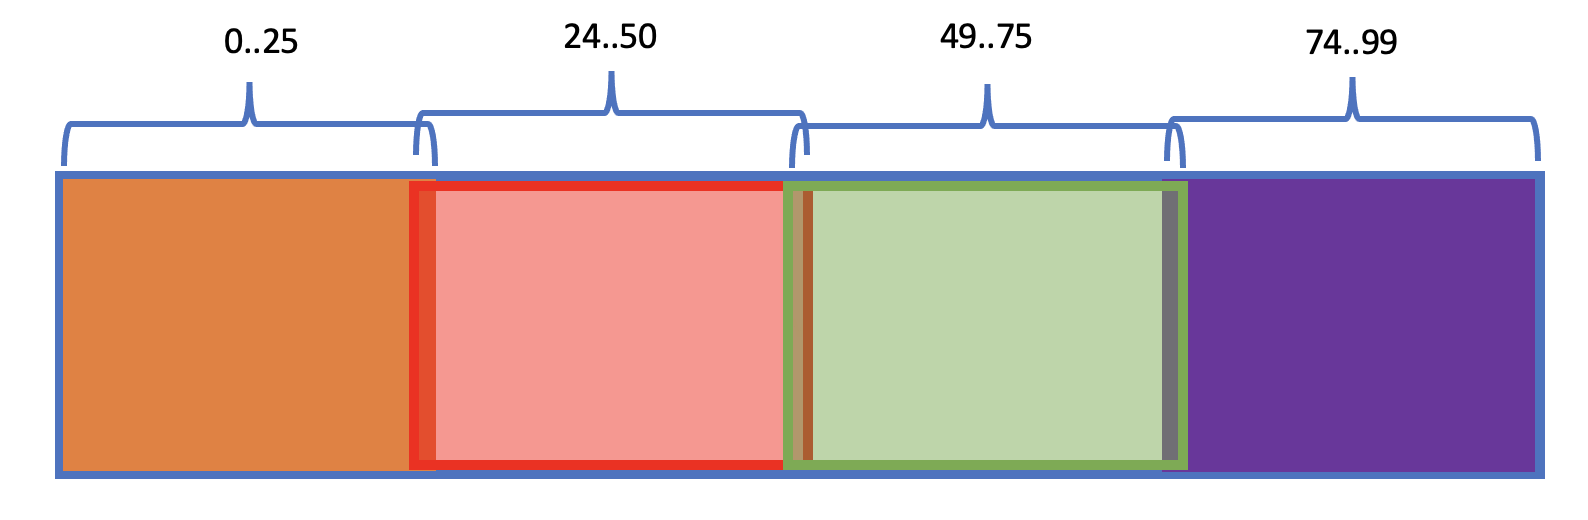
\includegraphics[height=1.5in]{figs/pbr.png}
  \caption{A blocked partition of a 1D region with ghost elements.}
  \label{fig:1dpbr}
\end{figure}

Another common partitioning idiom is to divide a region into blocks of the same size, a {\em blocked partitioning}.  For applications involving stencils, it can
also be useful for the blocks to include ``ghost cells'' adjacent to the block, essentially expanding the block in one or more dimensions.
Figure~\ref{fig:1dpbr} shows a 1D region partitioned into four subblocks, where each block includes one ghost element on each side.  For
a 1D region of 100 elements as shown in the figure, the result is four subblocks of size 26, 27, 27, and 26:  the two interior blocks have a ghost element on each side, while the first and last blocks have one ghost element each as the other element would be out of bounds of the region.

Figure~\ref{fig:pbr} gives code for computing the partitioning shown in Figure~\ref{fig:1dpbr}.  The essential differences from previous
  examples are on lines 21-27.  Starting with the {\tt create\_partition\_by\_restriction} call itself on line 27, we see that in addition to the
  usual context, index space, and color space this operation also takes a {\em transform} and an {\em extent}.  The extent $E$ is a ``generic''
  rectangle of the desired size---all subregions in the partition will have the shape of $E$.  The {\tt transform} $T$ is an
  $n \times m$ matrix, where $n$ is the number of dimensions of the color space and $m$ is the number of dimensions of the region.
  For a point $p$ in the color space, the points in the corresponding subregion are defined by the rectangle $Tp + E$.  That is $Tp$ defines
  an offset that is added to $E$ to name the points in the subregion associated with $p$.

  In this example, since the region and color space are both 1D, the transform is a 1x1 matrix, a single integer (lines 21-23); this transform
  says that subregions will start 25 elements apart (the {\tt blocksize}).  The extent defined on
  line 26 says that a subregion will extend one element to the left and 25 elements to the right of the 0-point of the subregion, so
  in general each subregion will have 27 elements.  Legion automatically clips any subregions that extend beyond the bounds of the region
  being partitioned, so for a color space of $\tt 0, 1, 2, 3$ the corresponding subregions will have elements $\tt 0..25, 24..50, 49..75, 74..99$.
  Note that unlike the other partitioning operations we have seen so far, the values of the color space are significant and affect the position
  of the subregion---for a region with an index space 0..99, it is necessary that the color space be $0..3$ and not some other set of four points.

\begin{figure}
  {\small
   \lstinputlisting[linerange={15-49}]{"Examples/Partitions/partition_by_restriction/pbr.cc"}
  }
  \caption{\legionbook{Partitions/partition\_by\_restriction/pbr.cc}}
  \label{fig:pbr}
\end{figure}


\section{Set-Based Partitions}
\label{sec:set}

Equal partitions, partitions by field and partitions by restriction are all examples of {\em independent} partitions, which are partitions that do
not depend on other partitions.  Legion also provides a number of {\em dependent} partitioning operators that take partitions as input and
produce partitions as output.  Dependent partitioning is used heavily in most Legion programs; it is not uncommon to see long chains of
partitioning operators to name complex subsets of the data that the program needs to manipulate. 

An {\em difference} partition takes two index space partitions and computes their set difference by color: A subspace of the difference partition
is the set difference of two subspaces, one from each of the two argument partitions, with the same color.  Thus, there is a subspace in the difference
partition for every color that the two argument partitions have in common.

Figure~\ref{fig:sets} gives an example that creates two partitions by restriction: a ``big'' partition that includes blocks of 26 elements spaced 25 elements apart (lines 22-28, similar to  the partition in Figure~\ref{fig:pbf} but with only one ghost element per subspace) and a ``small'' partition that is a disjoint partition of blocks of 25 elements spaced 25 elements apart (lines 22-24, 26, and 29). The region has 101 elements (line 6) to ensure that every subspace of the big partition actually has 26 elements (i.e., no elements are clipped for being out of bounds).  The difference partition subtracts the small partition from the big partition, so each subspace in the index partition names exactly the ghost element of the corresponding big subspace.  The result of the {\tt sum\_task} shows that there is exactly one element in each subregion of the difference partition.

Legion also provides {\tt create\_partition\_by\_union}, which
computes the set union of two partitions, and {\tt
  create\_partition\_by\_intersection}, which computes the set intersection
of two partitions.  These dependent
partitioning functions have the same signature as {\tt
  create\_partition\_by\_difference}.


\begin{figure}
  {\small
   \lstinputlisting[linerange={21-58}]{Examples/Partitions/sets/sets.cc}
  }
  \caption{\legionbook{Partitions/sets/sets.cc}}
  \label{fig:sets}
\end{figure}


\section{Image Partitions}
\label{sec:image}

\begin{figure}
  \centering
  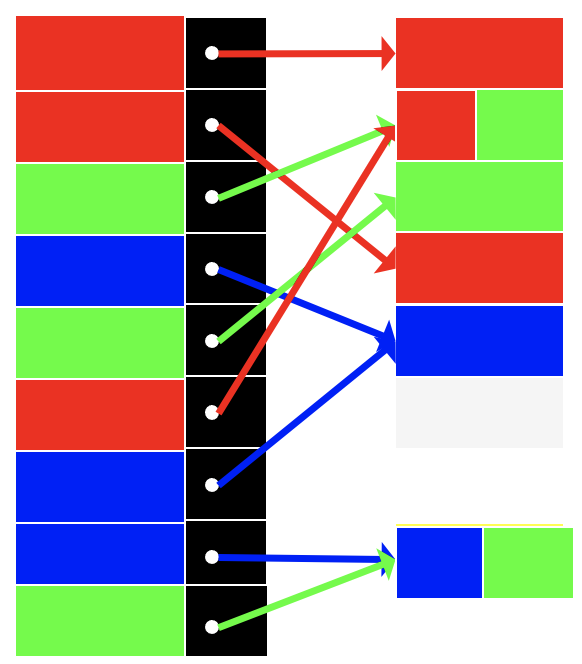
\includegraphics[height=2in]{figs/image.png}
  \caption{An image coloring.}
  \label{fig:eximage}
\end{figure}

  
Often we need to partition a region in a way compatible with an already computed partition of another region.
For example, consider a graph represented by a region of nodes and a region of edges. Assume we have chosen a partition of the nodes $\tt P_N[0],\ldots,P_N[k]$.
We will often want to partition the edges into subregions $\tt P_E[0],\ldots,P_E[k]$ such that the edges in $\tt P_E[i]$ all have source (or alternatively destination) nodes in $\tt P_N[i]$.  The {\em image} and {\em preimage} partitioning operators discussed in this section and the next provide mechanisms for using a pointer relationship between
two regions to induce a partitioning of one region given a partitioning of the other.

The example in Figure~\ref{fig:image} creates two regions.  The region {\tt lr\_src} (line 19) has a single field {\tt FIELD\_PTR} of type \verb+Point<1>+ (line 10).  Pointers
between regions are represented by points in the index space of the pointed-to region, which in this case is {\tt lr\_dst} (line 20).  The {\tt ptr\_task} (defined on lines 47-60 and called on lines 32-36) assigns pointers so that the $i$th element of {\tt lr\_src} points to the $i$th element of {\tt lr\_dst}.

The example creates an equal partition of {\tt lr\_src} on lines 29-30.  The {\tt create\_partition\_by\_image} ``transfers'' the partition of {\tt lr\_src} to the index space {\tt is}: if we think of the pointer field as a function from the source region to the destination index space and visualize the source partition as a coloring of the elements, then each pointer copies the color of its source element to the element of the destination.  An
example (unrelated to Figure~\ref{fig:image}) of taking the image of a pointer field under a partitioning of the source region is depicted in Figure~\ref{fig:eximage}.  In this abstract example, the coloring of the elements on the region on the left is copied via the pointer field to the elements of the index space or region on the right.  Because an element in the destination may have multiple pointers to it from the source, elements of the destination may have multiple colors, illustratedby the elements with two colors in Figure~\ref{fig:eximage}.  Thus, in general, the partition computed by {\tt create\_partition\_by\_image} may be aliased.  It may also be incomplete, as some elements of the destination region may have no pointers to them at all.  Because the pointer relationship is 1-1 between the source and destination regions
in the program in Figure~\ref{fig:image}, the partition of the destination in this case is both disjoint and complete.

The {\tt create\_partition\_by\_image} call on line 38 takes the current context, the index space to be partitioned, the source region partition, the source region, the identity of the pointer field in the source region, and the color space of the partition to be computed.  The result is an {\tt IndexPartition} of the destination index space.

The rest of the program (lines 41-45) sums the value field of the destination partition's subregions (which as in other examples has the same value 1 for every element).  Since the 1-1 pointer relationship copies the coloring exactly from source to destination and the source was an equal partition, the sums printed for each subregion are the same.

\begin{figure}
  {\small
    \lstinputlisting[linerange={17-76}]{Examples/Partitions/image/image.cc}
  }
  \caption{\legionbook{Partitions/image/image.cc}}
  \label{fig:image}
\end{figure}

\section{Pre-Image Partitions}
\label{sec:preimage}


\begin{figure}
  \centering
  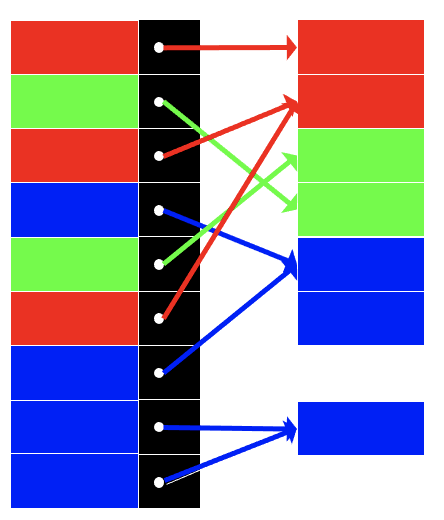
\includegraphics[height=2in]{figs/preimage.png}
  \caption{An preimage coloring.}
  \label{fig:expreimage}
\end{figure}

Where an image partition transfers a partitioning from a pointer's source region to its destination, a pre-image transfers a partitioning of the destination to the source.  Viewing
the pointer field as a function from source to destination, this operation is a preimage computation of that function.

The program in Figure~\ref{fig:preimage} gives an example.  As before there is a source region and a destination index space.  (Note that the source must be a region because
we need a pointer field, and only regions have fields.)  The source region has both the pointer field and the value field (lines 8-11), because we will be summing the subregions computed
by the preimage operation, which are subregions of the source region.  We do not need any fields in the destination region in this simple example, so its field space is empty (line 13).

Line 32 creates an equal partition {\tt ip\_dst} of the index space {\tt is} of the destination region.  The call to {\tt create\_partition\_by\_preimage} on line 35 transfers this partitioning backwards across the pointer field {\tt FIELD\_PTR} to the index space of the source region.  The call takes the current context, the partition of the destination index space, the source region, the source region's parent (or the source region itself if it has no parent, as in this example), the name of the pointer field in the source region, and the color space for the computed partition.

Figure~\ref{fig:expreimage} gives an abstract example of a preimage computation.  Here the pre-existing partition is on the right, and the color of each element is copied backwards through the pointer field to derive a coloring (a partitioning) of the source index space.  Note that because a pointer has a single source, a preimage is always guaranteed to be a disjoint partitioning of the source (but the partition may be incomplete---not every element of the source necessarily has a pointer into the destination).

Returning to the program in Figure~\ref{fig:preimage}, lines 38-43 sum the elements of the value field of each of the subregions of the source.  Again in this example the $i$th element of the source points to the $i$th element of the destination (lines 24-27 and 45-58), so the preimage operation replicates the equal partition of the destination in the source index space.  Since the value field is initialized to 1 (lines 21-22), the sums count the number of elements of each source subregion, which are all equal.


\begin{figure}
  {\small
   \lstinputlisting[linerange={17-74}]{"Examples/Partitions/pre_image/preimage.cc"}
  }
  \caption{\legionbook{Partitions/pre\_image/preimage.cc}}
  \label{fig:preimage}
\end{figure}


\chapter{Coherence}
\label{chap:coherence}

\section{Atomic}
\label{sec:atomic}

\section{Simultaneous}
\label{sec:simultaneous}




\chapter{Mapping}
\label{chap:mapping}
The Legion mapper interface is a key part
of the Legion programming system. Through the mapping interface applications
can control almost all decisions that can impact application performance.
The Legion philosophy is that these choices are better left to applications
rather than having heuristics in Legion that attempt to ``do the right thing'' in
every conceivable circumstance.  As a result, the very few performance heuristics
that are included in Legion are associated with low levels of the system
where there is no good way to expose those choices to the application.
For everything else the application must decide on the policy to use.

This design was chosen because of our own past experience with systems
where system heuristics did not behave as we desired, and we had no recourse
because those heuristics were not programmable by users.
Legion exposes these decisions so that expert programmers can achieve exactly
the effects they want, but it is also important to understand that squeezing every last bit of performance from a system may require understanding
and setting a wide variety of parameters exposed in the mapping interface.
This level of control can be overwheling at first to users who are not used to
considering all the possible dimensions that influence performance in complex,
distributed, and heterogeneous systems.

To help users write initial versions of their applications without needing
to concern themselves with tuning the performance knobs exposed by the mapper
interface, Legion provides a {\em default mapper}.  The default mapper
implements the Legion mapper API (like any other mapper) and provides a number
of heuristics that can provide reasonably performant, or at least correct, initial
settings.  However, it is unreasonable to expect the default mapper to provide excellent performance, and in
particular assuming that the performance of an application using the default
mapper is even an approximate indication of the performance that could be
achieved with a custom mapper is a mistake.


We will use several examples from the default mapper
to illustrate how mappers are constructed. We will also describe where
possible the heuristics that the default mapper employs to get 
reasonable performance. Because the default mapper uses generic heuristics
with no specific knowledge of the apllication, it is almost certain to make
poor decisions at least some of the time.
Performance benchmarking using only the default mapper is strongly
discouraged, while using custom application-specific mappers is
encouraged.  It is likely that the moment when you are dissatisfied with the 
heuristics in the default mapper will come sooner rather than later.
At that point the information in this chapter will be necessary for you
to write your own custom mapper, which might be as simple as
overriding a few features of the default mapper.

\section{Mapper Organization}
\label{sec:mapping:org}

The Legion mapper interface is an abstract C++ class that defines a set of 
pure virtual functions that the Legion runtime invokes as callbacks
for making performance-related decisions. A Legion mapper is therefore 
simply a class that inherits from the base abstract class and provides 
implementations of the associated pure virtual methods.

\subsection{Mapper Registration}
\label{subsec:mapping:registration}

After the Legion runtime is created, but before the application itself
begins, the application is given the opportunity to register mapper objects 
with the runtime. Figure~\ref{fig:mapper_registration} gives a small
example demonstrating how to register a custom mapper.

\begin{figure}
\begin{lstlisting}
void top_level_task(const Task *task,
		    const std::vector<PhysicalRegion> &regions,
		    Context ctx, 
		    Runtime *runtime)
{
  printf("Running top level task...\n");
}

class CustomMapperA : public DefaultMapper {
public:
  CustomMapperA(MapperRuntime *rt, Machine m, Processor p)
    : DefaultMapper(rt, m, p) { }
public:
  static void register_custom_mappers(Machine machine, Runtime *rt,
                                      const std::set<Processor> &local_procs);
};

/*static*/
void CustomMapperA::register_custom_mappers(Machine machine, Runtime *rt,
                                            const std::set<Processor> &local_procs)
{
  printf("Replacing default mappers with custom mapper A on all processors...\n");
  MapperRuntime *const map_rt = rt->get_mapper_runtime();
  for (std::set<Processor>::const_iterator it = local_procs.begin();
       it != local_procs.end(); it++)
    {
      rt->replace_default_mapper(new CustomMapperA(map_rt, machine, *it), *it);
    }
}

class CustomMapperB : public DefaultMapper {
public:
  CustomMapperB(MapperRuntime *rt, Machine m, Processor p)
    : DefaultMapper(rt, m, p) { }
public:
  static void register_custom_mappers(Machine machine, Runtime *rt,
                                      const std::set<Processor> &local_procs);
};

/*static*/
void CustomMapperB::register_custom_mappers(Machine machine, Runtime *rt,
                                            const std::set<Processor> &local_procs) 
{
  printf("Adding custom mapper B for all processors...\n");
  MapperRuntime *const map_rt = rt->get_mapper_runtime();
  for (std::set<Processor>::const_iterator it = local_procs.begin();
       it != local_procs.end(); it++)
    {
      rt->add_mapper(1/*MapperID*/, new CustomMapperA(map_rt, machine, *it), *it);
    }
}

int main(int argc, char **argv)
{
  Runtime::set_top_level_task_id(TOP_LEVEL_TASK_ID);
  {
    TaskVariantRegistrar registrar(TOP_LEVEL_TASK_ID, "top_level_task");
    registrar.add_constraint(ProcessorConstraint(Processor::LOC_PROC));
    Runtime::preregister_task_variant<top_level_task>(registrar);
  }
  Runtime::add_registration_callback(CustomMapperA::register_custom_mappers);
  Runtime::add_registration_callback(CustomMapperB::register_custom_mappers);

  return Runtime::start(argc, argv);
}
\end{lstlisting}
\caption{\legionbook{Mapping/registration/registration.cc}}
\label{fig:mapper_registration}
\end{figure}

To register {\tt CustomMapper} objects, the
application adds the mapper callback function by invoking the
{\tt Runtime::add\_registration\_callback} method, which takes as an
argument a function pointer to be invoked. The function pointer must
have a specific type, taking as arguments a {\tt Machine} object, 
a {\tt Runtime} pointer, and a reference to an STL set of {\tt Processor}
objects. The call can be invoked multiple times to record multiple
callback functions (e.g., to register multiple custom mappers). All
callback functions must be added prior to the invocation of the 
{\tt Runtime::start} method. We recommend that applications include the registration
method as a static method on the mapper class (as in Figure~\ref{fig:mapper_registration})
so that it is closely coupled to the custom mapper itself.

Before invoking any of the callback functions, the runtime 
creates an instance of the default mapper for each processor of
the system. The runtime then invokes the callback functions in the order
they were added. Each callback function is invoked once on each 
instance of the Legion runtime. For multi-process jobs, there will be 
one copy of the Legion runtime per process and therefore one invocation
of each callback per process. The set of processors passed into each 
registration callback function will be the set of application processors 
that are local to the process\footnote{Mappers cannot be associated with
utility processors, and therefore utility processors are not included
in the set.}, thereby providing a registration callback
function with the necessary context to know which processors it
will create new custom mappers for. 
If no callback functions are registered then the only mappers
that will be available are instances of the default mapper associated
with each application processor.

Upon invocation, the registration callbacks should create instances
of custom mappers and associate them with application processors. 
This step can be done through one of two runtime mapper calls. The mapper
can replace the default mappers (always registered with {\tt MapperID}
0) by calling {\tt Runtime::replace\_default\_mapper}, whichis the
only way to replace the default mappers. Alternatively, the registration
callback can use {\tt Runtime::add\_mapper} to register a mapper with a
new {\tt MapperID}. Both the {\tt Runtime::replace\_default\_mapper} and
the {\tt Runtime::add\_mapper} methods support an optional processor
argument, which tells the runtime to associate the mapper with a specific
processor. If no processor is specified, the mapper will be associated 
with all processors on the local node. This choice is mapper-specific:
whether one mapper object should handle a single application processor's
mapping decisions, or whether it should handle the mapping decisions for
all application processors on a node. Legion supports both use cases
and it is up to custom mappers to make the best choice. From a performance
perspective, the best choice is likely to depend on the mapper synchronization
model (see Section~\ref{subsec:mapping:sync}).

When creating custom mappers, the registration callback should get a pointer
to the {\tt MapperRuntime} and pass it as an argument to all mapper objects.
The mapper runtime will provide the interface for mapper calls to call back
into the runtime to acquire access to different physical resources. We 
will see instances of the use of the mapper runtime throughout the rest of
the examples in this chapter.

\subsection{Synchronization Model}
\label{subsec:mapping:sync}

Within an instance of the Legion runtime there are often several threads
performing the analysis necessary to advance the execution of an
application. If some threads are performing work for operations 
owned by the same mapper, it is possible that they will attempt to 
invoke mapper calls for the same mapper object concurrently. For both 
productivity and correctness reasons, we do not want users to be
responsible for making their mappers thread-safe. Therefore we allow
mappers to specify a {\em synchronization model} which the runtime will
follow when concurrent mapper calls are made.

Each mapper object can specify its own synchronization model via the
{\tt get\_mapper\_sync\_model} mapper call. The runtime invokes this
method exactly once per mapper object immediately after the mapper is
registered with the runtime. Once the synchronization model has been set
for a mapper object it cannot be changed. Currently three
synchronization models are supported:

\begin{itemize}
\item Serialized Non-Reentrant - Calls to the
      mapper object are serialized and execute atomically. If the mapper 
      calls out to the runtime and the mapper call is preempted, 
      no other mapper calls can be invoked by the runtime.
      This synchronization model conforms to the original version of
      the Legion mapper interface.
\item Serialized Reentrant - At most one mapper call
      executes at a time. However, if a mapper call invokes a runtime
      method that preempts the mapper call, the runtime may
      execute another mapper call or resume a previously blocked
      mapper call. It is up to the user to handle any changes in internal mapper
      state that might occur while a mapper call is preempted (e.g., the
      invalidation of STL iterators to internal mapper data structures).
\item Concurrent - Mapper calls to the same mapper object can
      proceed concurrently. Users can invoke the {\tt lock\_mapper} and
      {\tt unlock\_mapper} calls to perform their own synchronization
      of the mapper. This synchronization model is particularly useful for
      mappers that simply return static mapping decisions
      without changing internal mapper state.
\end{itemize}

The mapper synchronization offers mappers tradeoffs between mapper complexity and performance. The default mapper uses the 
serialized reentrant synchronization model as it offers a good trade-off
between programmability and performance.

\subsection{Machine Interface}
\label{subsec:mapping:machine}

All mappers are given a {\tt Machine} object to enable
introspection of the hardware on which the application is executing. The
{\tt Machine} object is a Realm-level object;  see {\tt realm/machine.h}.

There are two interfaces for querying the machine
object. The old interface contains methods such as {\tt get\_all\_processors}
and {\tt get\_all\_memories}. These methods populate STL data structures
with the appropriate names of processors and memories. We {\bf strongly}
discourage users from using these methods as they are not scalable on large
architectures with tens to hundreds of thousands of processors or memories.

The recommended, and more efficient and scalable, interface is based
on {\em queries}, which come in two types: {\tt ProcessorQuery} and 
{\tt MemoryQuery}. Each query is initially given a reference to the machine
object. After initialization the query lazily materializes the (entire) set of 
either processors or memories of the machine.
The mapper applies {\em filters} to the query to reduce the
set to processors or memories of interest.  These filters can include specializing
the query on the kind of processors with the {\tt only\_kind} method or by
requesting that the processor or memory have a specific affinity to another
processor or memory with the {\tt has\_affinity\_to}. Affinity can either be
specified as a minimum bandwidth or a maximum latency. Figure~\ref{fig:mapper_machine}
shows how to create a custom mapper that uses queries to find the local set of 
processors with the same processor kind as and the memories with affinities to the local
mapper processor. In some cases, these queries are still expensive, so we
encourage the creation of mappers that memoize the results of their most 
commonly invoked queries to avoid duplicated work.

\begin{figure}
\begin{lstlisting}
void top_level_task(const Task *task,
		    const std::vector<PhysicalRegion> &regions,
		    Context ctx, 
		    Runtime *runtime)
{
  printf("Running top level task...\n");
}

class MachineMapper : public DefaultMapper {
public:
  MachineMapper(MapperRuntime *rt, Machine m, Processor p);
public:
  static void register_machine_mappers(Machine machine, Runtime *rt,
                                       const std::set<Processor> &local_procs);
};

MachineMapper::MachineMapper(MapperRuntime *rt, Machine m, Processor p)
  : DefaultMapper(rt, m, p)
{
  // Find all processors of the same kind on the local node
  Machine::ProcessorQuery proc_query(m);
  // First restrict to the same node
  proc_query.local_address_space();
  // Make it the same processor kind as our processor
  proc_query.only_kind(p.kind());
  for (Machine::ProcessorQuery::iterator it = proc_query.begin(); 
        it != proc_query.end(); it++)
  {
    // skip ourselves
    if ((*it) == p)
      continue;
    printf("Mapper %s: shares " IDFMT "\n", get_mapper_name(), it->id);
  }
  // Find all the memories that are visible from this processor
  Machine::MemoryQuery mem_query(m);
  // Find affinity to our local processor
  mem_query.has_affinity_to(p);
  for (Machine::MemoryQuery::iterator it = mem_query.begin();
        it != mem_query.end(); it++)
    printf("Mapper %s: has affinity to memory " IDFMT "\n", get_mapper_name(), it->id);
}

/*static*/
void MachineMapper::register_machine_mappers(Machine machine, Runtime *rt,
                                             const std::set<Processor> &local_procs)
{
  printf("Replacing default mappers with custom mapper A on all processors...\n");
  MapperRuntime *const map_rt = rt->get_mapper_runtime();
  for (std::set<Processor>::const_iterator it = local_procs.begin();
       it != local_procs.end(); it++)
    {
      rt->replace_default_mapper(new MachineMapper(map_rt, machine, *it), *it);
    }
}

int main(int argc, char **argv)
{
  Runtime::set_top_level_task_id(TOP_LEVEL_TASK_ID);
  {
    TaskVariantRegistrar registrar(TOP_LEVEL_TASK_ID, "top_level_task");
    registrar.add_constraint(ProcessorConstraint(Processor::LOC_PROC));
    Runtime::preregister_task_variant<top_level_task>(registrar);
  }
  Runtime::add_registration_callback(MachineMapper::register_machine_mappers);

  return Runtime::start(argc, argv);
}
\end{lstlisting}
\caption{\legionbook{Mapping/machine/machine.cc}}
\label{fig:mapper_machine}
\end{figure}


\section{Mapping Tasks}
\label{sec:mapping:tasks}

\subsection{Task Placement}
\label{subsec:mapping:placement}

\subsection{Selecting Task Variants}
\label{subsec:mapping:variants}

\subsection{Creating Physical Instances}
\label{subsec:mapping:instances}

\subsection{Using Virtual Mappings}
\label{subsec:mapping:virtual}

\subsection{Profiling Requests}
\label{subsec:mapping:profiling}

\subsection{Resilience Support}
\label{subsec:mapping:resilience}



\section{Mapping Other Operations}
\label{sec:mapping:others}

\subsection{Mapping Copies}
\label{subsec:mapping:copies}

\subsection{Mapping Acquires and Releases}
\label{subsec:mapping:acquires}

\subsection{Mapping Must Epoch Launches}
\label{subsec:mapping:mustepoch}



\section{Managing Execution}
\label{sec:mapping:execution}

\subsection{Context Management}
\label{subsec:mapping:context}

\subsection{Mapper Communication}
\label{subsec:mapping:communication}

\subsection{Controlling Stealing}
\label{subsec:mapping:stealing}


\chapter{Interoperation}
\label{chap:interop}

In this chapter we briefly discuss the most common scenarios where Legion programs need to interoperate with other systems.  We will rely in this chapter on examples from the {\tt legion/examples} directory in the Legion repository.

\section{MPI}
\label{sec:mpi}

Legion has well-developed support for interoperation with MPI.  The essentials of the approach are:
\begin{itemize}
\item The top-level Legion task is control-replicated, with a number of shards equal to the number of ranks of MPI.
\item Legion and MPI time-slice the machine:  One of MPI or Legion is running at any given time, while the other runtime
  waits.
\item Data can be shared between MPI and Legion by attaching an MPI buffer as a region with simultaneous coherence (with the correct layout constraint
  to ensure the buffer contents are interpreted correctly by Legion).  The data can be moved back and forth between a shard of the top-level
  task and the corresponding MPI rank using the producer-consumer synchronization discussed in Section~\ref{sec:simultaneous}.
\end{itemize}

MPI interoperation is illustrated in {\tt legion/examples/mpi\_with\_ctrl\_repl/mpi\_with\_ctrl\_repl.cc}:
  \begin{lstlisting}
    MPILegionHandshake handshake;
    ...
    // This is the preferred way of using handshakes in Legion                                                                                                                                                                                                                               
    IndexLauncher worker_launcher(WORKER_TASK_ID, launch_bounds, TaskArgument(NULL, 0), args_map);
    // We can use our handshake as a phase barrier                                                                                                                                                                                                                                          
    // Record that we will wait on this handshake    
    worker_launcher.add_wait_handshake(handshake);
    // Advance the handshake to the next version
    handshake.advance_legion_handshake();
    // Then record that we will arrive on this version
    worker_launcher.add_arrival_handshake(handshake);
    // Launch our worker task
    // No need to wait for anything
    runtime->execute_index_space(ctx, worker_launcher);
  \end{lstlisting}
In this excerpt, we see that the synchronization between MPI and Legion is wrapped in a {\tt MPILegionHandshake} object (line 1).  The handshake encapsulates a phase barrier and is used similarly (see Section~\ref{sec:simultaneous}), but a handshake also knows how to work with MPI.
An index task launcher is built to run the Legion-side work (line 4) and its execution is deferred until the MPI side signals it is done running (line 7).  Just like a phase barrier, handshakes have generations so that they can be reused multiple times, typically across
iterations of a loop.  The handshake is advanced to the next generation (line 9) and when the index tasks are finished the (new generation of the) handshake is signaled to restart the MPI side (line 11).

The MPI side of the interface is symmetric.  From the same example:
\begin{lstlisting}
  for (int i = 0; i < total_iterations; i++)
  {
    printf("MPI Doing Work on rank %d\n", rank); // MPI work goes here
    if (strict_bulk_synchronous_execution)
       MPI_Barrier(MPI_COMM_WORLD);
    // Perform a handoff to Legion, this call is 
    // asynchronous and will return immediately
    handshake.mpi_handoff_to_legion();
    ..
    // Wait for Legion to hand control back,
    // This call will block until a Legion task
    // running in this same process hands control back
    handshake.mpi_wait_on_legion();
    if (strict_bulk_synchronous_execution)
      MPI_Barrier(MPI_COMM_WORLD);
  }
\end{lstlisting}
MPI uses the same handshake object as Legion.  Note that the
call to {\tt mpi\_wait\_on\_legion} blocks until Legion arrives at the handshake; the other arrive/wait handshake methods are asynchronous.
Because the MPI side blocks while it is waiting on Legion, it is not concerned with the generation of the handshake, so the generation should only be
advanced by the Legion side to allow for deferred execution of Legion tasks.


\section{OpenMP}
\label{sec:openmp}

Legion provides a straightfoward model of interoperation with OpenMP.  Legion tasks may use OpenMP pragmas internally to exploit
multiple threads in a single kernel.  Legion tasks that use OpenMP should be mapped to OMP processors, which can be enforced by
adding an OMP  constraint when the task is registered.

Under the hood Legion interoperates with OpenMP by directly implementing OpenMP functionality.  Only a subset of OpenMP is supported,
but the support extends to the most commonly used features, particularly {\tt omp parallel for}.

The program {\tt legion/omp\_saxpy} illustrates typical uses of OpenMP in Legion programs.  In this code, the leaf tasks (the tasks
that do not call other tasks) include OpenMP pragmas.  For example, in {\tt simple\_blas.cc} a dot product operation is defined:
\begin{lstlisting}
template <>
float BlasTaskImplementations<float>::dot_task_cpu(const Task *task,
						   const std::vector<PhysicalRegion> &regions,
						   Context ctx, Runtime *runtime)
{
  IndexSpace is = regions[1].get_logical_region().get_index_space();
  Rect<1> bounds = runtime->get_index_space_domain(ctx, is);

  const FieldAccessor<READ_ONLY,float,1,coord_t,
          Realm::AffineAccessor<float,1,coord_t> > fa_x(regions[0], task->regions[0].instance_fields[0]);
  const FieldAccessor<READ_ONLY,float,1,coord_t,
          Realm::AffineAccessor<float,1,coord_t> > fa_y(regions[1], task->regions[0].instance_fields[0]);

  float acc = 0;
#\##pragma omp parallel for reduction(+:acc) if(blas_do_parallel)
  for(int i = bounds.lo[0]; i <= bounds.hi[0]; i++)
    acc += fa_x[i] * fa_y[i];
  return acc;
}
\end{lstlisting}
Note that unlike most other examples in this manual, this code uses an {\tt AffineAccessor} for the fields.  Affine accessors support indexing into regions like arrays, which is necessary in this example because the different
iterations of the loop will be split across multiple OpenMP threads---we cannot use an iterator here, as an iterator by definition defines a sequential order of access to the elements iterated over.  The {\tt axpy} task in the same file gives another example of using
OpenMP pragmas within Legion tasks.

The code for registering the tasks that use OpenMP is in {\tt simple\_blas.inl}:
\begin{lstlisting}
  {
    dot_task_id = Runtime::generate_static_task_id();
    TaskVariantRegistrar tvr(dot_task_id);
#\##ifdef REALM_USE_OPENMP
    tvr.add_constraint(ProcessorConstraint(Processor::OMP_PROC));
#\##else
    tvr.add_constraint(ProcessorConstraint(Processor::LOC_PROC));
#\##endif
    Runtime::preregister_task_variant<T, BlasTaskImplementations<T>::dot_task_cpu>(tvr, "dot (cpu)");
  }
\end{lstlisting}
This code is parameterized on whether OpenMP is to be used or not; if it is used the processor constraint for the task is set to {\tt OMP\_PROC}, otherwise it is set to {\tt LOC\_PROC} (i.e., CPUs).

There are a few command-line flags that affect the execution of Legion programs using OpenMP:
\begin{itemize}

\item {\tt -ll:ocpus n} sets the number of CPUs to be reserved for OpenMP to $n$.
\item {\tt -ll:othr t} sets the njmber of threads per CPU to $t$.
\item {\tt -ll:okindhack} exposes the master OpenMP thread as a CPU processor. This flag is useful when running with {\tt -ll:cpus 0} to give an extra processor to the OpenMP runtime; if there are some remaining CPU tasks they can be sent to the
    procesor running the master OpenMP thread using {\tt -ll:okindhack}.
\item {\tt -ll:onuma} ensures that OpenMP cores are grouped by NUMA domain; a warning is printed if NUMA support is not found.
\item {\tt -ll:ostack m} sets the OpenMP stack size to $m$ bytes.
\end{itemize}

Finally, Legion is not compiled with OpenMP by default.  To enable OpenMP, build Legion with {\tt USE\_OPENMP = 1}.
  

\section{HDF5}
\label{sechdf5}

\section{Kokkos}
\label{sec:kokkos}

\section{Python}
\label{sec:python}

\part{Reference}

\section{High Level Runtime}

\section{Tasks}

\section{Task Launchers}

\section{Futures}

\section{Regions}

\section{Partitions}


\bibliographystyle{alpha}
\bibliography{bibliography}

\end{document}
